\setcounter{chapter}{1}
\setchapterabstract{This chapter discusses vertical foreclosure under Article 102 TFEU, where dominant firms leverage power in a primary market to exclude competition in a secondary market. Firms may engage in vertical foreclosure to protect dominance, maximize profits, or achieve efficiency. Practices such as refusal to deal can restrict access to essential inputs, potentially stifling innovation and investment. Conditions for forced sharing include indispensability of resources and lack of objective justification. Margin squeeze and tying involve manipulating input prices or product bundling to restrict competition downstream. Finally, self-preferencing, highlighted in the Google Shopping case, involves a dominant firm favouring its own products to secure a competitive edge in adjacent markets, potentially influencing consumer behaviour and limiting competition}
\chapter{Vertical Foreclosure}
\vspace{-1.5cm}

\setcounter{chapter}{12}
{\chaptoc\noindent\begin{minipage}[inner sep=0,outer sep=0]{0.9\linewidth}\section*{The landmark scenario}\end{minipage}}

\begin{figure}[ht]
    \centering
    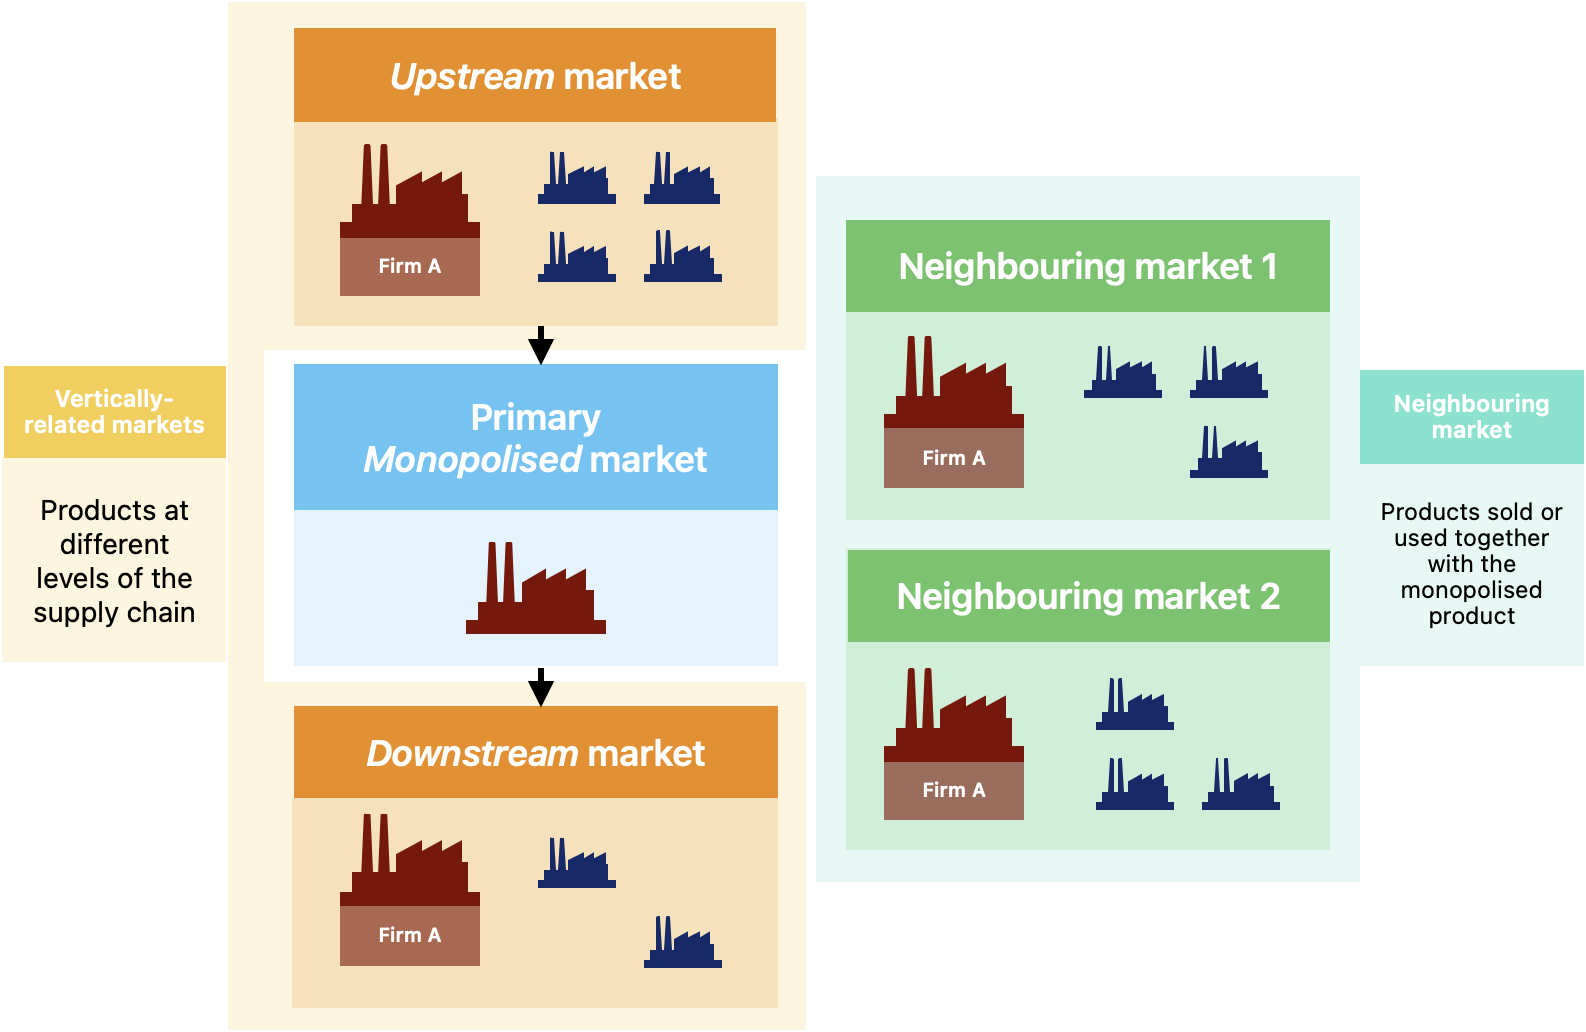
\includegraphics[width=0.75\linewidth]{image12-1.png}
\end{figure}

\section{Vertical Foreclosure}

    \Definition{
    Dominant firm \textbf{leverages its dominance/uses its market power} in the primary market \textbf{to restrict competition} (i.e. to exclude firms competing with it) in a secondary market
    }{Vertical Foreclosure}

    The following sections provide a brief overview as to why a firm would have incentives to engage in such practices.

\newpage
    \subsection{Shelter dominance}
    \subsubsection*{Indirect effect on primary market}

        Exclude firms from secondary markets to protect the dominant position in the primary market from being challenged by actual or potential rivals that may expand. 
        
        The monopolist may act to restrict competition in secondary markets to avoid firms becoming successful there, and then leveraging their position achieved in the secondary market to challenge/compete more aggressively/expand in the primary market.

    \subsection{Maximize profits}
    \subsubsection*{Effect on secondary market}

        In regulated markets, where the dominant firm can only charge a fixed price (lower than the monopoly price) on the primary market, by monopolizing the secondary market the dominant firm can make monopoly profits there.
        
        Even if there is no price cap, the dominant firm may want to expand its dominance (and thus its monopoly profits) to a related market. 
        
        The dominant firm uses/leverages its success (or a legal monopoly) in the primary market to obtain rewards (monopoly profits) in a market where it would not be as successful without the abuse

        \Remark{This behaviour may harm competition, increase prices and reduce consumer welfare in the secondary market}

    \subsection{Enhance efficiency}
    \subsubsection*{Objective justifications}

        Dominant firms may combine their strength in the primary market with their position in the secondary market to:
        
        \begin{itemize}
            \item Avoid double marginalization (in vertically related markets) or the Cournot effect (in neighbouring markets, where the price of one product influences demand for the other) by internalizing a pricing externality through bundling.
            \item Price discriminate, thereby increasing allocative efficiency.
            \item Reduce costs or achieve efficiencies (e.g., economies of scope).
            \item Defend product quality (when products are used together).
        \end{itemize}

        \Remark{Pro-competitive justifications that the defendant may use to show that its practice does not harm consumer welfare}

\section{Refusal to deal}

        \subsubsection{Definition}

            \Definition{A dominant firm that is vertically-integrated (or active in neighbouring markets) refuses to supply rivals in a secondary market (in which it is not dominant) with an input they need to compete in that secondary market.}{Refusal to deal}

            Forcing a dominant firm to share the required upstream input with its downstream rivals may have potentially detrimental effects on competition:

            \begin{itemize}
                \item It may reduce the dominant firm’s incentive to (create or) improve the input (e.g., spending on innovation and maintenance) as rivals would take advantage of the investments.
                \item It could incentivize laziness among non-dominant firms, discouraging competing investments in innovation. Rivals might free-ride on the dominant firm’s efforts instead of investing to create better alternatives, opting to “wait and see” and, if the innovation is successful, obtain it through antitrust.
                \item It may incentivize cooperation between rivals.
                \item It could force courts or authorities to act like ‘central planners.’
            \end{itemize}

        \subsubsection{Conditions for a refusals to deal to be anticompetitive}

            A dominant firm can be forced to share its proprietary resources when:
            
            \begin{enumerate}
                \item \textbf{Indispensability:} The refused resource is objectively indispensable (and not duplicable) to compete in the downstream or upstream market (i.e., it is an ‘essential facility’).
                \begin{itemize}
                    \item Termination of an existing relationship is more likely to be abusive if a customer made specific investments to use the input, making the input more likely to be indispensable.
                    \item Refusal is likely to eliminate all effective competition (including innovation) in the secondary market on the part of the entity requesting access to the product or service. Competitors retaining a marginal presence in certain niches is not sufficient.
                    \item “An undertaking which has a dominant position in the market in raw materials and […] refuses to supply a customer, which is […] a manufacturer of […] derivatives, and therefore risks eliminating all competition on the part of this customer, is abusing its dominant position.” (Commercial Solvents)
                    \item “[W]here a dominant undertaking refuses to give access to an infrastructure that it has developed for the needs of its own business, […] obliging that undertaking to grant access cannot be justified […] unless the dominant undertaking has a genuinely tight grip on the market concerned.” (Slovak Telekom)
                \end{itemize}
                \item \textbf{No objective justification:} The refusal does not pursue a legitimate interest (other than excluding a competitor) of the dominant undertaking, or the conduct is disproportionate.
            \end{enumerate}

        \subsubsection{Some clarifications}

            \textbf{Indispensability.} An input is indispensable if competition downstream cannot take place without using that input, there is no actual or potential substitute, and timely duplication is impossible. This condition is not required if the firm is under a legal obligation to give access.

            \begin{itemize}
                \item \textbf{Physical.} E.g., ports and airports for carriers, national railway infrastructure for national railway operators, or national gas pipelines for gas producers.
                \item \textbf{Legal.} E.g., intellectual property rights (copyright or patent) owned by the dominant undertaking.
                \item \textbf{Economical.} The market is not sufficiently large to sustain a second facility similar to the dominant firm’s system.
            \end{itemize}
            
            \textbf{Objective justifications.} For example, in a credit card system, an objective justification for refusing to provide a credit card or to admit a bank to the system could be the lack of anti-fraud security devices or the fact that the customer is a bad debtor. For pipelines, an objective justification could be capacity constraints.
            
            \begin{itemize}
                \item If the relationship was ongoing, supplying the input does not imply a risk that the owner of the input will receive inadequate compensation for its investment.
            \end{itemize}

        \subsubsection{Refusal to license IP}

        \begin{itemize}
            \item The Commission applies the same factors to a refusal to license IP rights as to other types of refusal to supply.
            \item In the case of IP, it is also required that the refusal is likely to block technical development or a new market—i.e., the Commission may require dominant firms to share their IP rights only to ensure innovative products are brought to the market or rivals are able to produce follow-on innovations for which there is potential consumer demand. It is not sufficient to simply duplicate the goods or services already offered.
            \item The Commission considers itself able to make an ex post and case-by-case analysis of a certain pattern of incentives, even though in so doing it runs the risk of overturning what national IP legislators chose and over-deterring lawful conducts.
            \item US courts’ approach is more lenient—US enforcers generally reject any intrusion when IP is involved.
        \end{itemize}


\newpage
        \subsubsection{The strange case of Constructive Refusal / Access Restrictions}

        Both a ‘plain and simple’ refusal and a ‘constructive refusal’ (i.e., an offer to supply on unreasonable terms) can be abusive.

        \begin{itemize}
            \item However, finding an abuse in cases involving a constructive refusal to deal, or any case other than a plain, outright refusal (anything more than a “no”), requires much less stringent criteria.
            \item In particular, the EU Courts and the European Commission found that “access restrictions,” referring to the imposition by a dominant undertaking of restrictions on access to an input other than a refusal to supply, do not have to meet the specific legal test discussed above.
            \item Access restrictions can be abusive even if the input is not indispensable, as the need to protect the undertaking’s freedom of contract and incentives to invest does not apply to the same extent as in a refusal to supply setting.
            \begin{itemize}
                \item This includes cases where the input is (i) financed by public funds, (ii) not owned by the dominant firm, (iii) subject to a regulatory obligation to give access, or (iv) offered to the same or other third parties, now or in the past (then interrupted, degraded, or delayed).
            \end{itemize}
            \item The importance or indispensability of the input will increase the likelihood of exclusionary effects.
        \end{itemize}

\section{Margin squeeze}

        \subsubsection{Definition}

            \Definition{A vertically integrated firm, dominant upstream, supplies a key input to competitors downstream, at a price that affects their ability to compete. By charging a high price for the input, the dominant firm squeezes the margin available downstream making it impossible for the rival downstream to compete}{Margin squeeze}

            \begin{itemize}
                \item More efficient competitors downstream may have to exit when the price of the upstream input increases, while the dominant firm can compensate for the losses downstream with the margin upstream, and future margin downstream once the as-efficient (or more efficient) competitors are excluded.
                \item It is not necessary to establish that the upstream input is indispensable.
                \item However, the more important the input is to effectively compete downstream, the more likely the exclusionary effects.
            \end{itemize}

            \Remark{The same conduct can be constructive refusal to deal, excessive price of input or predatory price of downstream product}

        \subsubsection{Test}

            If the dominant firm’s captive business paid the External Supply Price and charged the Retail Price, would it be able to cover the long run average incremental costs (LRAIC) of its downstream operations?

            \begin{figure}[ht]
                \centering
                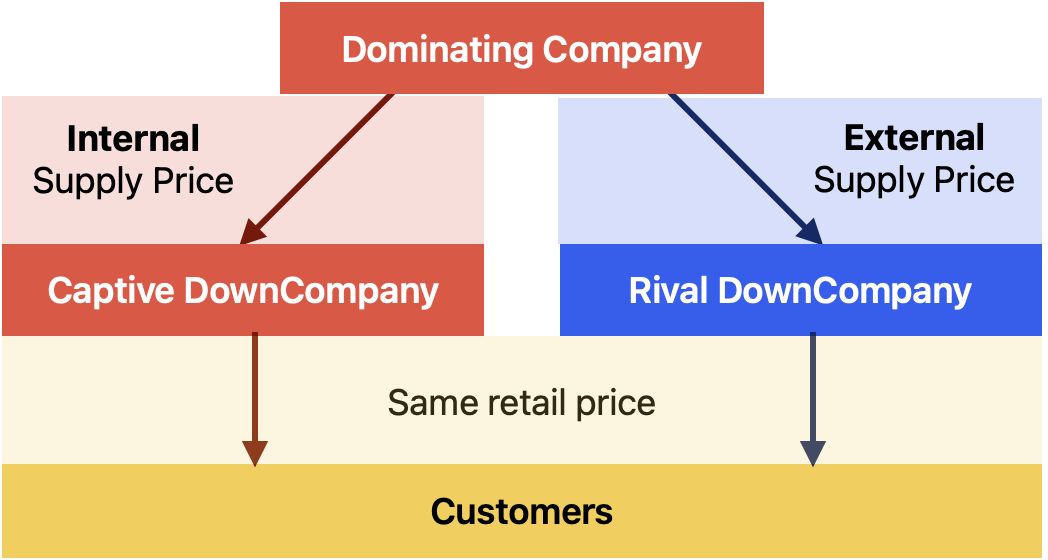
\includegraphics[width=0.5\linewidth]{image12-2.png}
            \end{figure}
            
        \subsubsection{Characteristics of the price charged} 

            \begin{itemize}
                \item To be abusive, \textbf{the price charged} by the dominant firm for the input \textbf{must leave an insufficient margin} for the downstream competitors to compete (in the sale of the downstream product).
                \item \textbf{The insufficient margin is the essence of the abuse}. The Commission generally relies on the LRAIC of the dominant firm’s downstream operations to determine whether it has squeezed the margin available to an equally-efficient competitor\sn{\Note{The Commission may use the costs of a downstream competitor where it is not possible to calculate the costs of a vertically-integrated dominant firm.}}. 
                \item A clear case of margin squeeze is when the dominant firm charges a price for the input that is higher than or equal to the retail price it charges for the downstream product.
            \end{itemize}
      
\section{Tying}

        \subsubsection{Definition}

            \Definition{The (dominant) supplier of the tying product requires customers to source from it also a second and separate product, the tied product (on which it is not normally dominant) as a package.}{Tying}

            \begin{itemize}
                \item It is \textbf{tying/pure bundling} when the products can be purchased only together (i.e., the two products are not supplied by the dominant firm individually).
                \begin{itemize}
                    \item The dominant firm forces customers to get two products together, even when the two could have been sold separately.
                    \item The dominant firm refuses to supply the tying product (i.e., the product that the customer wants) unless the customer also purchases/receives the tied product with it (which it would not necessarily get from the same firm otherwise).
                    \item This can happen through contractual obligations (\textbf{contractual tying}) or as a result of technical integration/incompatibility\sn{\Note{\textbf{technological tying}, i.e., one product comes integrated with the other—for example, Microsoft selling Windows OS with Windows Media Player and Internet Explorer}}.
                \end{itemize}
                \item It is \textbf{mixed bundling} (or \textbf{commercial tying}) when the products are also available separately, but the sum of their individual prices is higher than the bundle price.
            \end{itemize}

        \subsubsection{Two “distinct” products}

            Selling a car with its tires (or shoes with shoelaces) is not tying, except if extended to the aftermarket. The products must be considered distinct. For example, it is tying when the purchaser of a car is forced to insure it only with a certain insurance company.

            Two products are distinct (and thus potentially subject to tying) if, in the absence of tying, a substantial number of customers would purchase the tying product without purchasing the tied product from the same supplier (i.e., there is separate customer demand for the tied product). There might be evidence that customers purchase tying and tied products separately or that manufacturers sell the tied product without the tying one.
            
            Consider the following factors:
            \begin{enumerate}
                \item nature and technical features of the products,
                \item customers’ and competitors’ behaviour,
                \item history of development of the products,
                \item commercial practice of the dominant undertaking.
            \end{enumerate}
            
            Tying is often an aftermarket issue. For example, requiring the use of only Xerox paper with Xerox copiers, or in the \textbf{Hilti nail cartridges case}: the requirement that users of Hilti’s patented nail cartridges must also acquire nails from Hilti is tying because the nail gun (1), the cartridge strip (2), and the nails (3) are three distinct products.

            \Remark{Independent producers should be free to manufacture consumables (nails) intended for use in equipment manufactured by others unless in doing so they would infringe IP rights.}

        \subsubsection{Effects}

            When can we consider it more likely that tying has a foreclosure effect (and thus amounts to anticompetitive abusive conduct)?
            
            \begin{enumerate}
                \item If the tying strategy is long-lasting, for example through technical tying, which is costly to reverse.
                \item If the firm is dominant (or has strong market power) in more than one of the products in the bundle. The greater the number of such products in the bundle, the more likely the anti-competitive foreclosure, as the bundle is difficult for a competitor to replicate, either on its own or in combination with others.
                \item If consumer inertia or bias in the tied market is significant.
                \item If the tied product is an important complementary product for customers of the tying product (or a material share of customers in the tied market also purchase the tying product). With the reduction of alternative suppliers of the tied product, entry into the tying market becomes more difficult.
                \item If there are significant barriers to entry or expansion in the tied market (e.g., need to achieve economies of scale or scope, presence of network effects).
            \end{enumerate}

        \subsubsection{Objective justifications}

            \begin{enumerate}
                \item \textbf{Economic efficiencies}, e.g., lower costs of production, packaging and distribution, transport and transaction costs, economies of scale/scope.
                \item \textbf{Control of product quality, safety, security}, and the dominant firm’s goodwill.
                \item \textbf{Better efficiency of the tying product} when used with the tied product\sn{\Note{for example, certain equipment may function at its best only if a particular material or component is used, which is available solely from the manufacturer.}}.
                \item \textbf{Network effects}: selling more of the tying and tied products may make both more useful or valuable for consumers.
                \item \textbf{Discrimination between} (e.g., high-volume and low-volume) \textbf{customers}: when the tied products are complements, tying may be used to charge consumers with a high willingness to pay more, while others may afford to use it at a lower package price, as seen in “products as a service” models (e.g., printers, papers, and toners).
                \item \textbf{Cournot effect}: when the price of one of the tied goods increases, consumers demand a lower quantity of both.\sn{\Note{the monopolist is incentivized not to charge a double margin on the two products, but a single margin on the bundle.}}
            \end{enumerate}

\section{Bundling rebates}

        \subsubsection{Definition}

            \Definition{achieve the same effect as a tying agreement through pricing practices – a rebate on the combination of two or more products.\marginnote{\Example{
            For example, Rossignol produces not only skis but also bindings, and charges a discounted price for the bundle of its products (skis + bindings):
            \[P_{ski} = 5\]
            \[P_{bindings} = 10\]
            \[P_{ski+bindings} = 12\]
            The rebate regards two products/markets. Let’s assume, for the sake of the analysis, that Rossignol has a dominant position in skis, while the market for bindings is competitive.
            }}}{Bundling rebates}

        \subsubsection{Liability for bundle rebates}

            \begin{itemize}
                \item \textbf{First scenario:} Rivals of the dominant firm produce all the products in the bundle. Thus, a bundle can compete against another bundle.
                \begin{itemize}
                    \item Antitrust enforcers check whether the “price of the bundle as a whole” is predatory. In other words, they establish if:
                    \begin{itemize}
                        \item either \( P(\text{Sk} + \text{B}) < AVC_{\text{Sk}} + AVC_{\text{B}} \)
                        \item or \( AVC_{\text{Sk}} + AVC_{\text{B}} < P(\text{Sk} + \text{B}) < ATC_{\text{Sk}} + ATC_{\text{B}} \) with evidence of exclusionary intent
                    \end{itemize}
                \end{itemize}
                \item \textbf{Second scenario:} Rivals produce only bindings, not skis.
                \begin{itemize}
                    \item Given that \( P_{\text{Sk}} = 5 \), \( P_{\text{B}} = 10 \), and \( P(\text{Sk} + \text{B}) = 12 \), the price that the rivals have to charge for their bindings to match the bundle rebate is:
                    \begin{itemize}
                        \item Since they cannot modify the price for skis (\( P_{\text{Sk}} = 5 \)),
                        \item They must charge \( P_{\text{B}} \leq 7 \) to compete with the bundle price. In other words, they must shift the amount of the whole discount (\( 15 - 12 = 3 \)) onto the only product they “control” (bindings), pushing their price down to \( 10 - 3 = 7 \).
                    \end{itemize}
                \end{itemize}
            \end{itemize}


\section{Self-preferencing}

        \subsubsection{A new kind of abuse}

        It is a “new” type of abuse, typified (indirectly) in the Google Shopping case and in the latest draft 102 guidelines by the European Commission.
    
        \Definition{\textbf{Self-preferencing} consists of a dominant undertaking actively giving preferential treatment to its own products compared to those of competitors, mainly by means of non-pricing behaviour.}{Self-preferencing}
        
        The dominant undertaking leverages its dominance in a given market (the “leveraging” market) to gain an advantage in a related market (the “leveraged” market) by means of preferential treatment of its product in the leveraged market. Self-preferencing may involve positioning or displaying the leveraged product in the leveraging market, manipulating consumer behaviour and choice, or manipulating auctions. 
        
        The preferential treatment departs from competition on the merits when it:
        \begin{itemize}
            \item (i) takes place in a leveraging market that constitutes an important source of business for competitors in the leveraged market, which competitors cannot effectively replace through other means;
            \item (ii) is likely to influence the behaviour of users;
            \item (iii) is likely contrary to the business rationale of the dominant firm in the leveraging market, e.g., contrary to its interests or those of its customers.
        \end{itemize}

        
    